\documentclass[border=4pt]{standalone}
% Shared typography and colours for the standalone figures.
\usepackage{unicode-math}
\setmainfont{TeX Gyre Heros}
\setmathfont{TeX Gyre Pagella Math}
\usepackage{tikz}
\usetikzlibrary{arrows.meta,positioning,calc,decorations.pathreplacing}
\usepackage{pgfplots}
\pgfplotsset{compat=1.18}

% One colour per element or subsystem. Record the mapping in
% the working repository conventions and use it identically in every figure.
\definecolor{elemA}{HTML}{1F5FA8}
\definecolor{elemB}{HTML}{B8461B}
\definecolor{elemC}{HTML}{2E7D32}
\definecolor{elemD}{HTML}{6A4C93}
\definecolor{frameline}{HTML}{555555}

\begin{document}
\hyphenpenalty=10000
\exhyphenpenalty=10000
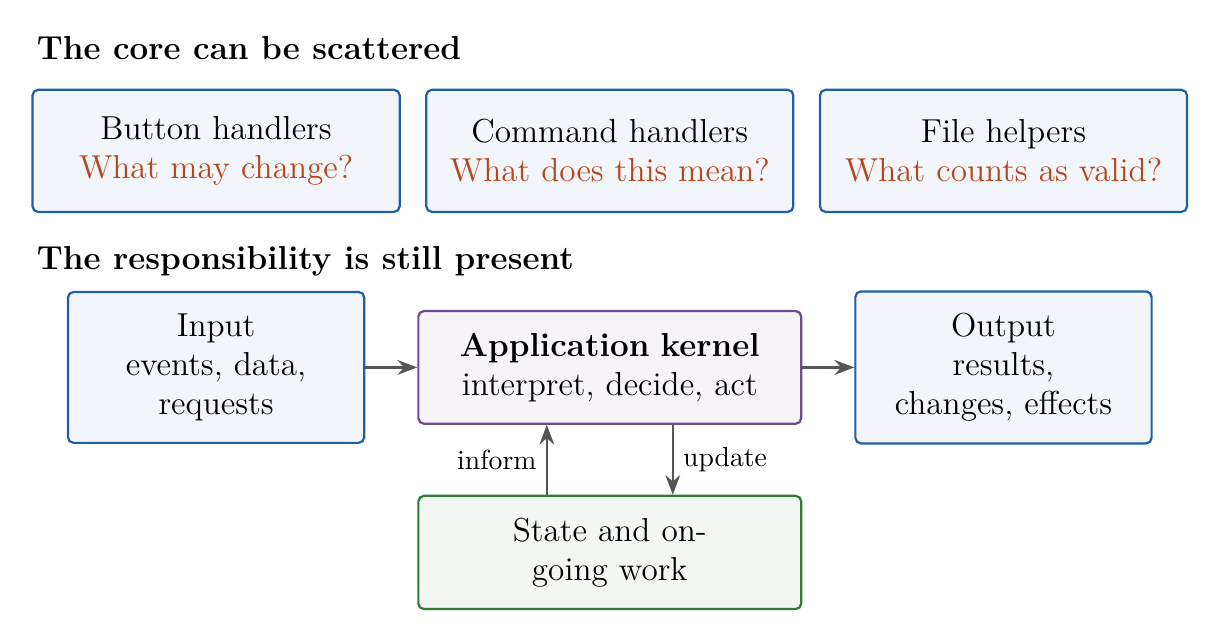
\begin{tikzpicture}[
  box/.style={draw,rounded corners=2pt,thick,align=center,inner sep=8pt,font=\large},
  surface/.style={box,draw=elemA,fill=elemA!6,text width=4.1cm,minimum height=1.55cm},
  arrow/.style={-{Stealth[length=2.5mm]},thick,draw=frameline}
]
\node[font=\large\bfseries,anchor=west] at (-7.4,3.6) {The core can be scattered};
\node[surface] (gui) at (-5,2.3) {Button handlers\\\textcolor{elemB}{What may change?}};
\node[surface] (cmd) at (0,2.3) {Command handlers\\\textcolor{elemB}{What does this mean?}};
\node[surface] (file) at (5,2.3) {File helpers\\\textcolor{elemB}{What counts as valid?}};
\node[font=\large\bfseries,anchor=west] at (-7.4,0.9) {The responsibility is still present};
\node[box,draw=elemA,fill=elemA!6,text width=3.2cm,minimum height=1.4cm] (in) at (-5,-0.45)
  {Input\\events, data, requests};
\node[box,draw=elemD,fill=elemD!6,text width=4.3cm,minimum height=1.4cm] (core) at (0,-0.45)
  {\textbf{Application kernel}\\interpret, decide, act};
\node[box,draw=elemA,fill=elemA!6,text width=3.2cm,minimum height=1.4cm] (out) at (5,-0.45)
  {Output\\results, changes, effects};
\draw[arrow] (in) -- (core);
\draw[arrow] (core) -- (out);
\node[box,draw=elemC,fill=elemC!6,text width=4.3cm] (state) at (0,-2.8)
  {State and ongoing work};
\draw[arrow] ([xshift=-8mm]state.north) -- node[left,font=\normalsize] {inform} ([xshift=-8mm]core.south);
\draw[arrow] ([xshift=8mm]core.south) -- node[right,font=\normalsize] {update} ([xshift=8mm]state.north);
\end{tikzpicture}
\end{document}
